\chapter{CC-Inclusive Cross Section Selection Filter} \label{ch:meas}

One of the cross-section measurements MicroBooNE can make is an inclusive charged-current cross-section measurement (referred to as CC-inclusive). CC-inclusive events consist of a neutrino exchanging a $W^{\pm}$ boson with an argon atom, producing a charged lepton and any number of other final state particles. In MicroBooNE's case, a CC-inclusive event will mostly have a defining muon track coming out of the vertex due to our neutrinos being predominately $\nu_{\mu}$s. A cross-section measurement is the energy dependent probability of $\nu-Ar$ interaction in the detector. Cross-sections however are independent of the intensity or focus of the particle beam so they can be compared among different experiments. A background for a CC-inclusive cross-section measurement are the neutral-current events that contain a pion. It is possible to have a neutral current interaction with a $\pi+p$ event signature that looks like a charged current $\mu+p$ event. Reconstruction tools implemented to date don't efficiently separate muons from pions. A common way to separate these two particles species is to implement a track length cut. On average, muons tend to have longer track lengths in LArTPCs so by requiring that the hypothesized lepton be above a threshold track length, it is possible to increase signal to background.

MicroBooNE requires fully automated event reconstruction and selection algorithms for use in the many physics measurements being worked on to date due to the large data rate MicroBooNE receives. Being able to automatically pluck out the neutrino interaction among a sea of cosmics proved to be challenging but was accomplished. MicroBooNE has developed two complementary and preliminary selection algorithms to select charged-current $\nu_{\mu}-Ar$ interactions. Both are fully automated and cut based. The results below focus on the first selection and the ``In-Progress'' plots presented on the poster associated with this proceeding will focus on further improving this algorithm using Convolutional Neural Network (CNN) implementations. The full details can be found in MicroBooNE public note \cite{ccinclusive} and for more information of CNN implementation on MicroBooNE data refer to \cite{cnn}. Selection I is based on cuts developed in a MC performance study described in \cite{mcccinclusive}. It identifies the muon from a neutrino interaction without biasing towards track multiplicity. To combat cosmic and neutral current background, the analysis is strongly biased towards forward-going long tracks which are contained. This limits phase space and reduces acceptance. 

The efficiency and purity are used as performance values of selection I. Efficiency is described as the number of selected true $\nu_{\mu}$ CC events divided by the number of expected true $\nu_{\mu}$ CC events. The purity is described as the number of selected true $\nu_{\mu}$ CC events divided by the sum of itself and all the backgrounds. The efficiency of selection I is 12\% and the purity is 39.7\%. The poster related to this proceedings will focus on the last cut which requires the longest track to be longer than 75 cm. This cut has a passing rate of 30\% w.r.t the previous cut and is implemented in part to separate charged-current events from neutral-current events that mimic our signal. Implementing a CNN for $\mu-\pi$ separation picks out differences in these two particles that are track range independent therefore eliminating the need for the 75 cm track length cut and increase efficiency and passing rate at low muon momentum. Figure \ref{fig:track} shows the track distribution of selection I and the lack of data below  the 75 cm track length cut. Figure \ref{fig:eff} shows the efficiency of selection I as a function of muon momentum.     
The selection begins with a cut that requires an optical flash greater than 50 photo electrons (PE) in the 1.6 $\mu$s beam window. Next, two or more 3D reconstructed tracks must be within 5 cm from a 3D reconstructed vertex. The most forward going track vertex-track association is then selected for further cuts. The vertex from the chosen association must be in the fiducial volume, and the longest track from this association must be matched to a flash 80 cm in z. Lastly the longest track must be contained and longer than 75 cm.       

\begin{figure}[htp!]
\centering
	\begin{subfigure}[b]{.4\textwidth}
	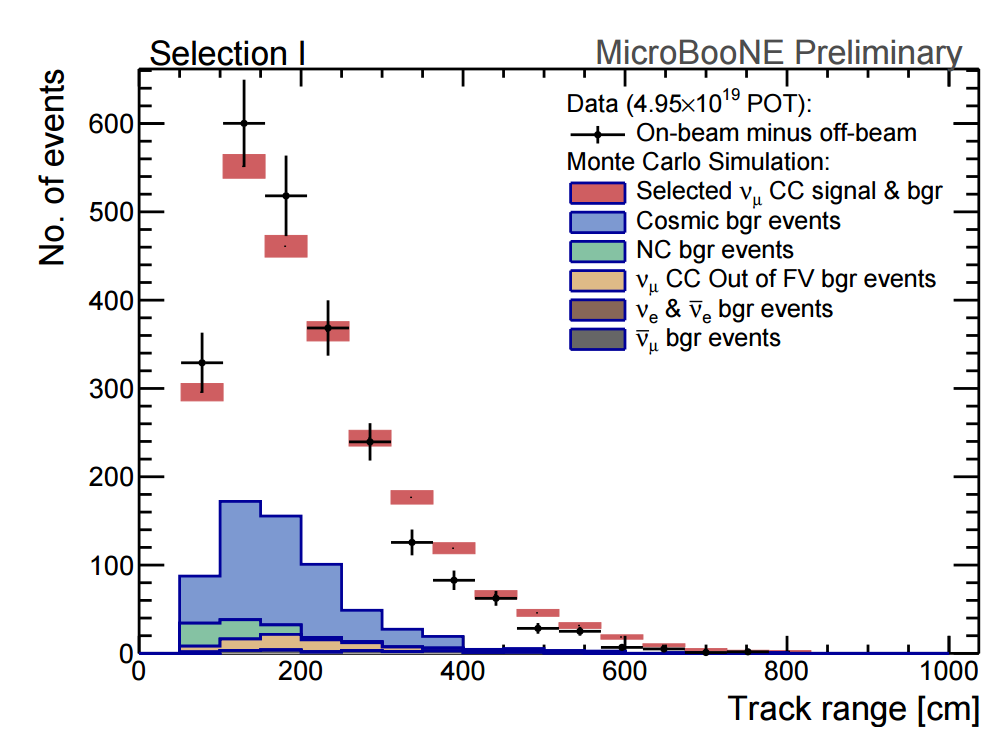
\includegraphics[width=\textwidth]{figs/track_distribution.png}
	\caption{Track range distribution of selection I}
	\label{fig:track}
	\end{subfigure}
	\quad	
	\begin{subfigure}[b]{.4\textwidth}
	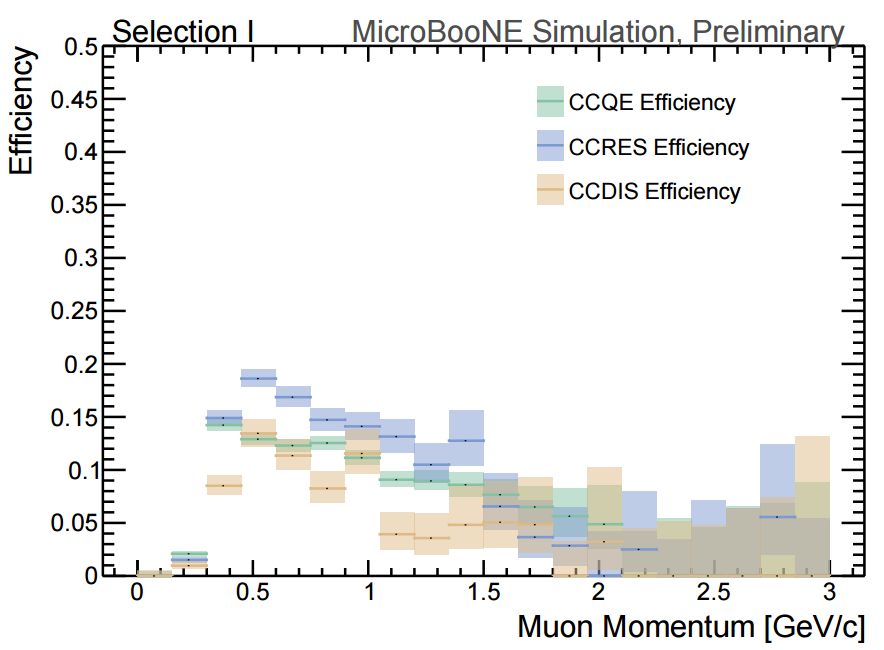
\includegraphics[width=\textwidth]{figs/efficiencyvsmom.png}
	\caption{Selection efficiency as a function of the true muon momentum}
	\label{fig:eff}
	\end{subfigure}
	\quad
\label{fig:distributions}
\caption{\ref{fig:track} Track range distribution for selection I. The track range is defined as the 3D distance between the start and end of the muon candidate track. No data is shown below 75 cm due to the track length cut described previously. \ref{fig:eff} Efficiency of the selected events by process quasi-elastic (QE), resonant (RES), and deep-inelastic (DIS). Statistical uncertainty is shown in the bands and the distributions are a function of true muon momentum. The rise of the efficiency between 0 GeV and 0.5 GeV is due to the minimum track length cut and the decreasing efficiency for higher momentum tracks is caused by the containment requirement.} 
\end{figure}
